\documentclass[10pt,a4paper]{article}

\usepackage[margin=1.05in]{geometry}
\usepackage{setspace,amsmath,amssymb,amsthm}
\usepackage{graphicx,enumitem,titlesec,fancyhdr,microtype,booktabs}
\usepackage{hyperref}
\hypersetup{colorlinks=true,linkcolor=black,urlcolor=black,citecolor=black}
\graphicspath{{../../drawings/pass1/walk/}{../../drawings/pass2/}}

\titleformat{\section}{\normalsize\bfseries}{}{0em}{}
\titlespacing*{\section}{0pt}{1.35em}{0.5em}

\theoremstyle{plain}
\newtheorem{proposition}{Proposition}
\theoremstyle{definition}
\newtheorem{definition}{Definition}
\theoremstyle{remark}
\newtheorem{observation}{Observation}

\setstretch{1.14}
\pagestyle{fancy}
\fancyhf{}
\fancyhead[L]{\small\itshape Elements of Position}
\fancyhead[R]{\small\itshape II.\ Without an Angle}
\fancyfoot[C]{\small\thepage}
\renewcommand{\headrulewidth}{0pt}

\begin{document}

\begin{center}
\vspace*{2.0em}
{\large Elements of Position}\\[1.5em]
{\LARGE\bfseries II.\ Without an Angle}\\[0.5em]
{\small Two moves, the pair they force, and two mixes that must not be crushed}\\[1.6em]
{\normalsize Justin Erholtz}\\[0.3em]
{\small 24 September 2026}
\end{center}

\vspace{1.2em}

\begin{center}
{\large The operators do not contain the joint.}
\end{center}

\vspace{1.0em}

\noindent
\textit{A note.}
Part~I named the pair on the integer and the lock at \(n=1\).
This part walks.
Identities of the pair are citations of Part~I.
A gap, a word, a mean taken over one run, are reported from a named table.
The recorded run is
\texttt{kernels/walk/runs/2026-09-24\_h0.002\_n200000/}:
\(h=0.002\), \(200{,}000\) steps, \(H_0=1571\), \(127\) hits.
That summary is byte-identical to the \(19\)~September record.
A different kick writes a new table.
It does not revise an identity.

\vspace{0.5em}
\noindent
\textit{A note on names.}
Shear \(T_h\), bind \(N\), step, hit, heading \(u_m\).
Outer point \(P_m=m u_m\). Inverse point \(Q_m=u_m/m\).
Half-turn mix --- \(h=\tan(\pi/n)\).
Vertex mix --- \(h=\tan(2\pi/n)\).
These two mixes are not one sentence.

\tableofcontents

\section{The operators}

Start on the diameter: \((1,0)\).

\begin{definition}[Shear]
\(T_h(x,y)=(x-hy,\; y+hx)\) for \(h>0\).
\end{definition}

\begin{definition}[Bind]
\(N(x,y)=(x,y)/\sqrt{x^2+y^2}\).
\end{definition}

\begin{definition}[Step]
\(\mathrm{step}=N\circ T_h\).
\end{definition}

No angle is an argument of either move.
Composed, one step is a rotation by \(\arctan h\).
That identity is classical (Volder, \(1959\)).
It is never used inside the walk.
It is used only to name a comparison after a table exists.

\begin{definition}[Hit]
A hit is a step at which the heading's second coordinate changes sign.
\end{definition}

On the recorded run the first hit is step \(H_0=1571\), heading
\((-0.99999992,\;-0.00040316)\).
The same first crossing, at the same \(h\), is what the continuous-clock reading counts as its half-turn \(H\).
Two detectors, one event.

\begin{figure}[htbp]
\centering
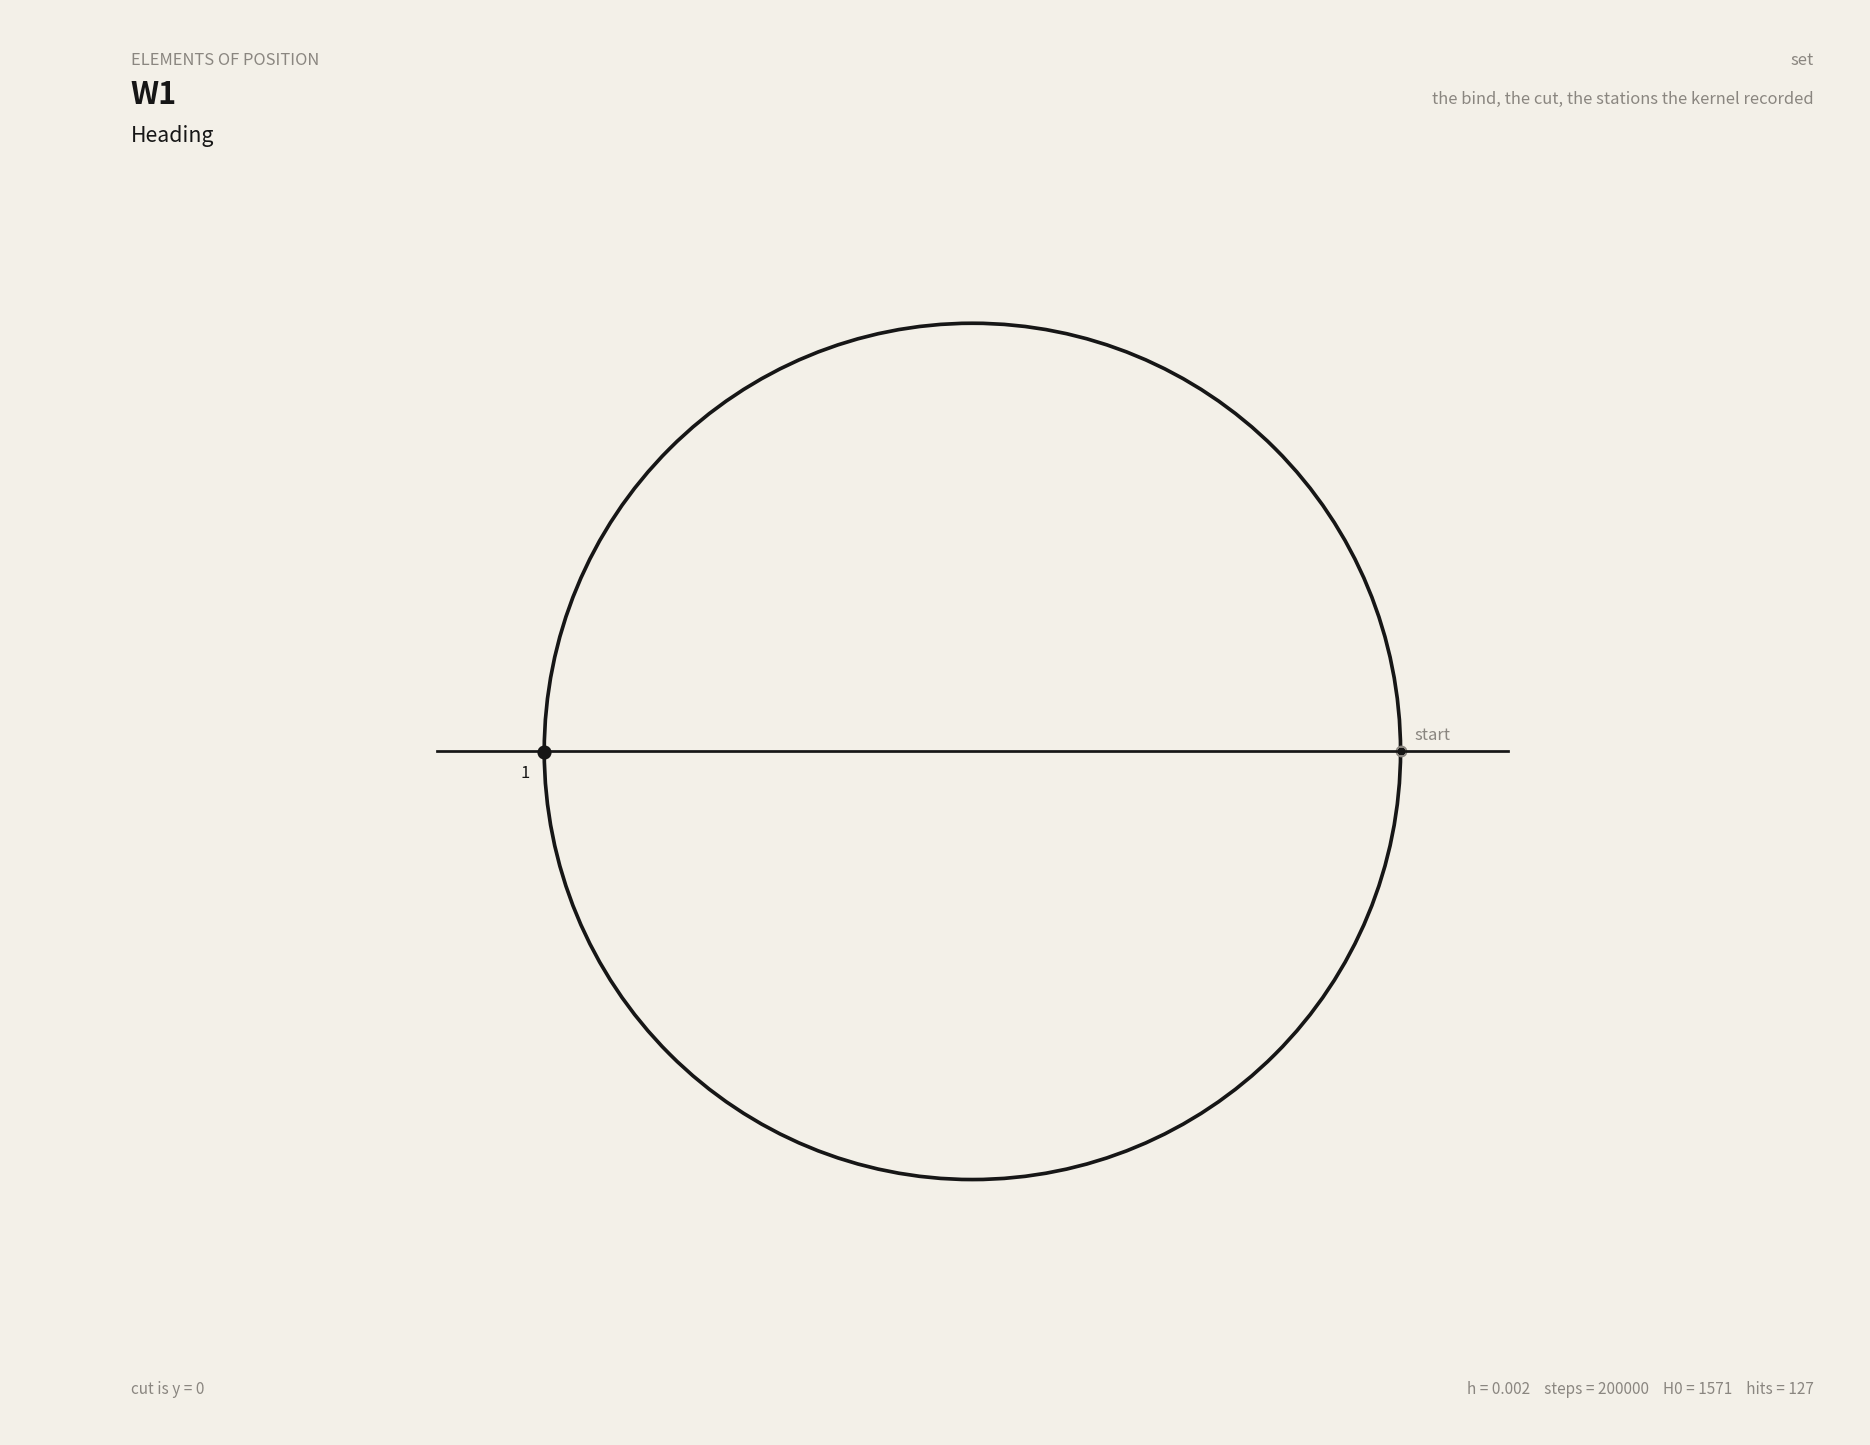
\includegraphics[width=0.92\textwidth]{W1_heading.png}
\caption{Sheet W1. The bind, the cut, the stations the kernel recorded.}
\end{figure}

\section{The pair is already proved}

Once the hit index \(m\) is named, Part~I applies with \(n=m\).

\[
r\cdot\frac1r=1,\qquad
\mathrm{GM}=1,\qquad
\tau(m)=\frac{(m-1)^2}{2m}.
\]

\(P_m=m u_m\) and \(Q_m=u_m/m\) are that pair read as points on the recorded ray.
\(Q_m\) is the inversion of \(P_m\) through the bind:
\(|P_m|^2=m^2\), so \(P_m/|P_m|^2=Q_m\).

\begin{figure}[htbp]
\centering
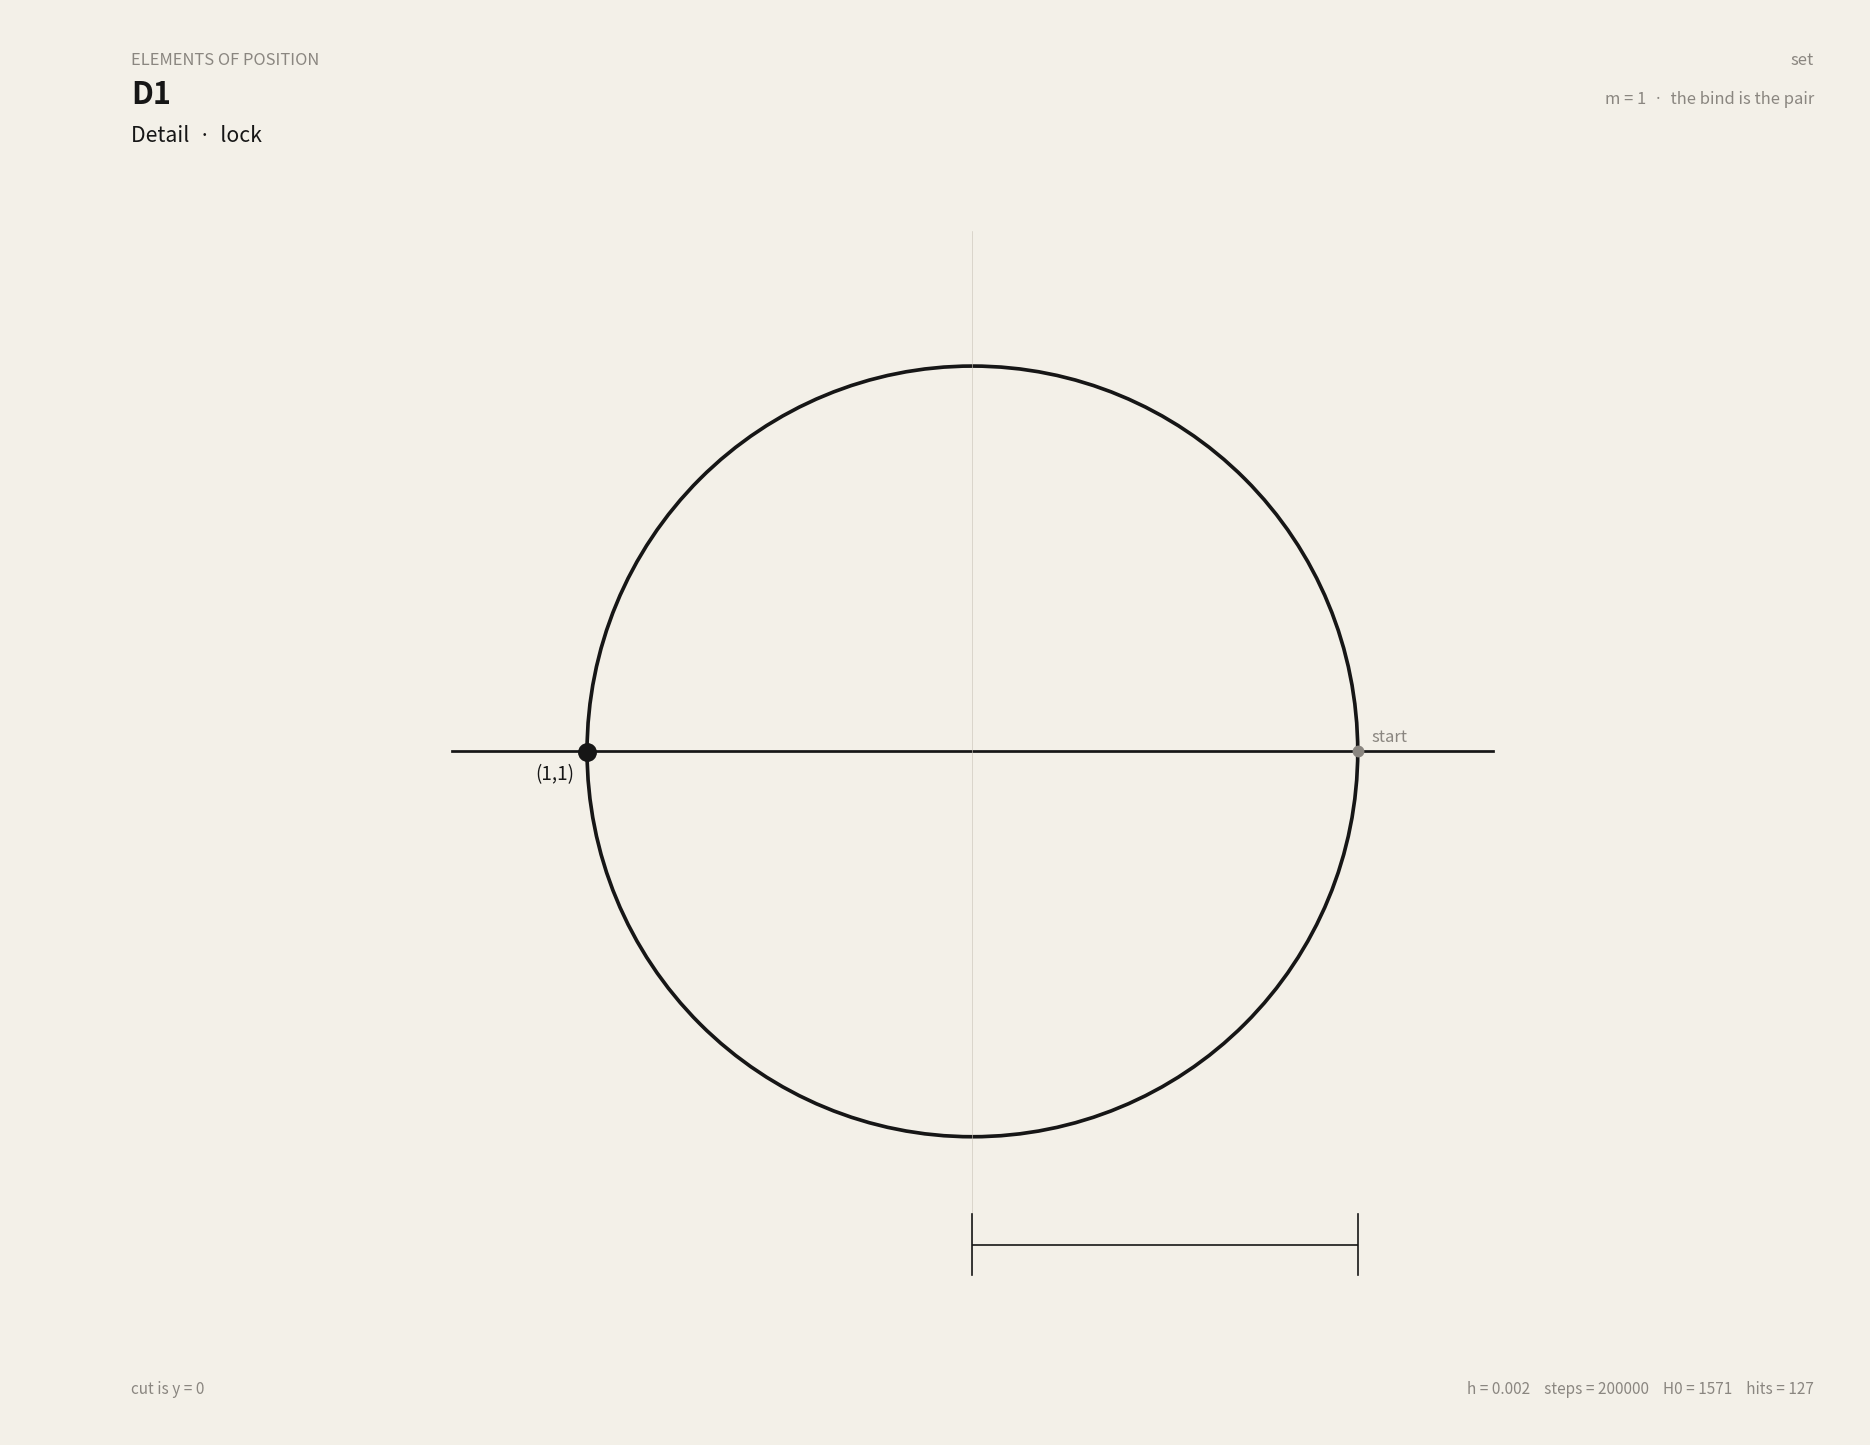
\includegraphics[width=0.92\textwidth]{D1_lock.png}
\caption{Sheet D1. The lock. Pair \((1,1)\).}
\end{figure}

\begin{figure}[htbp]
\centering
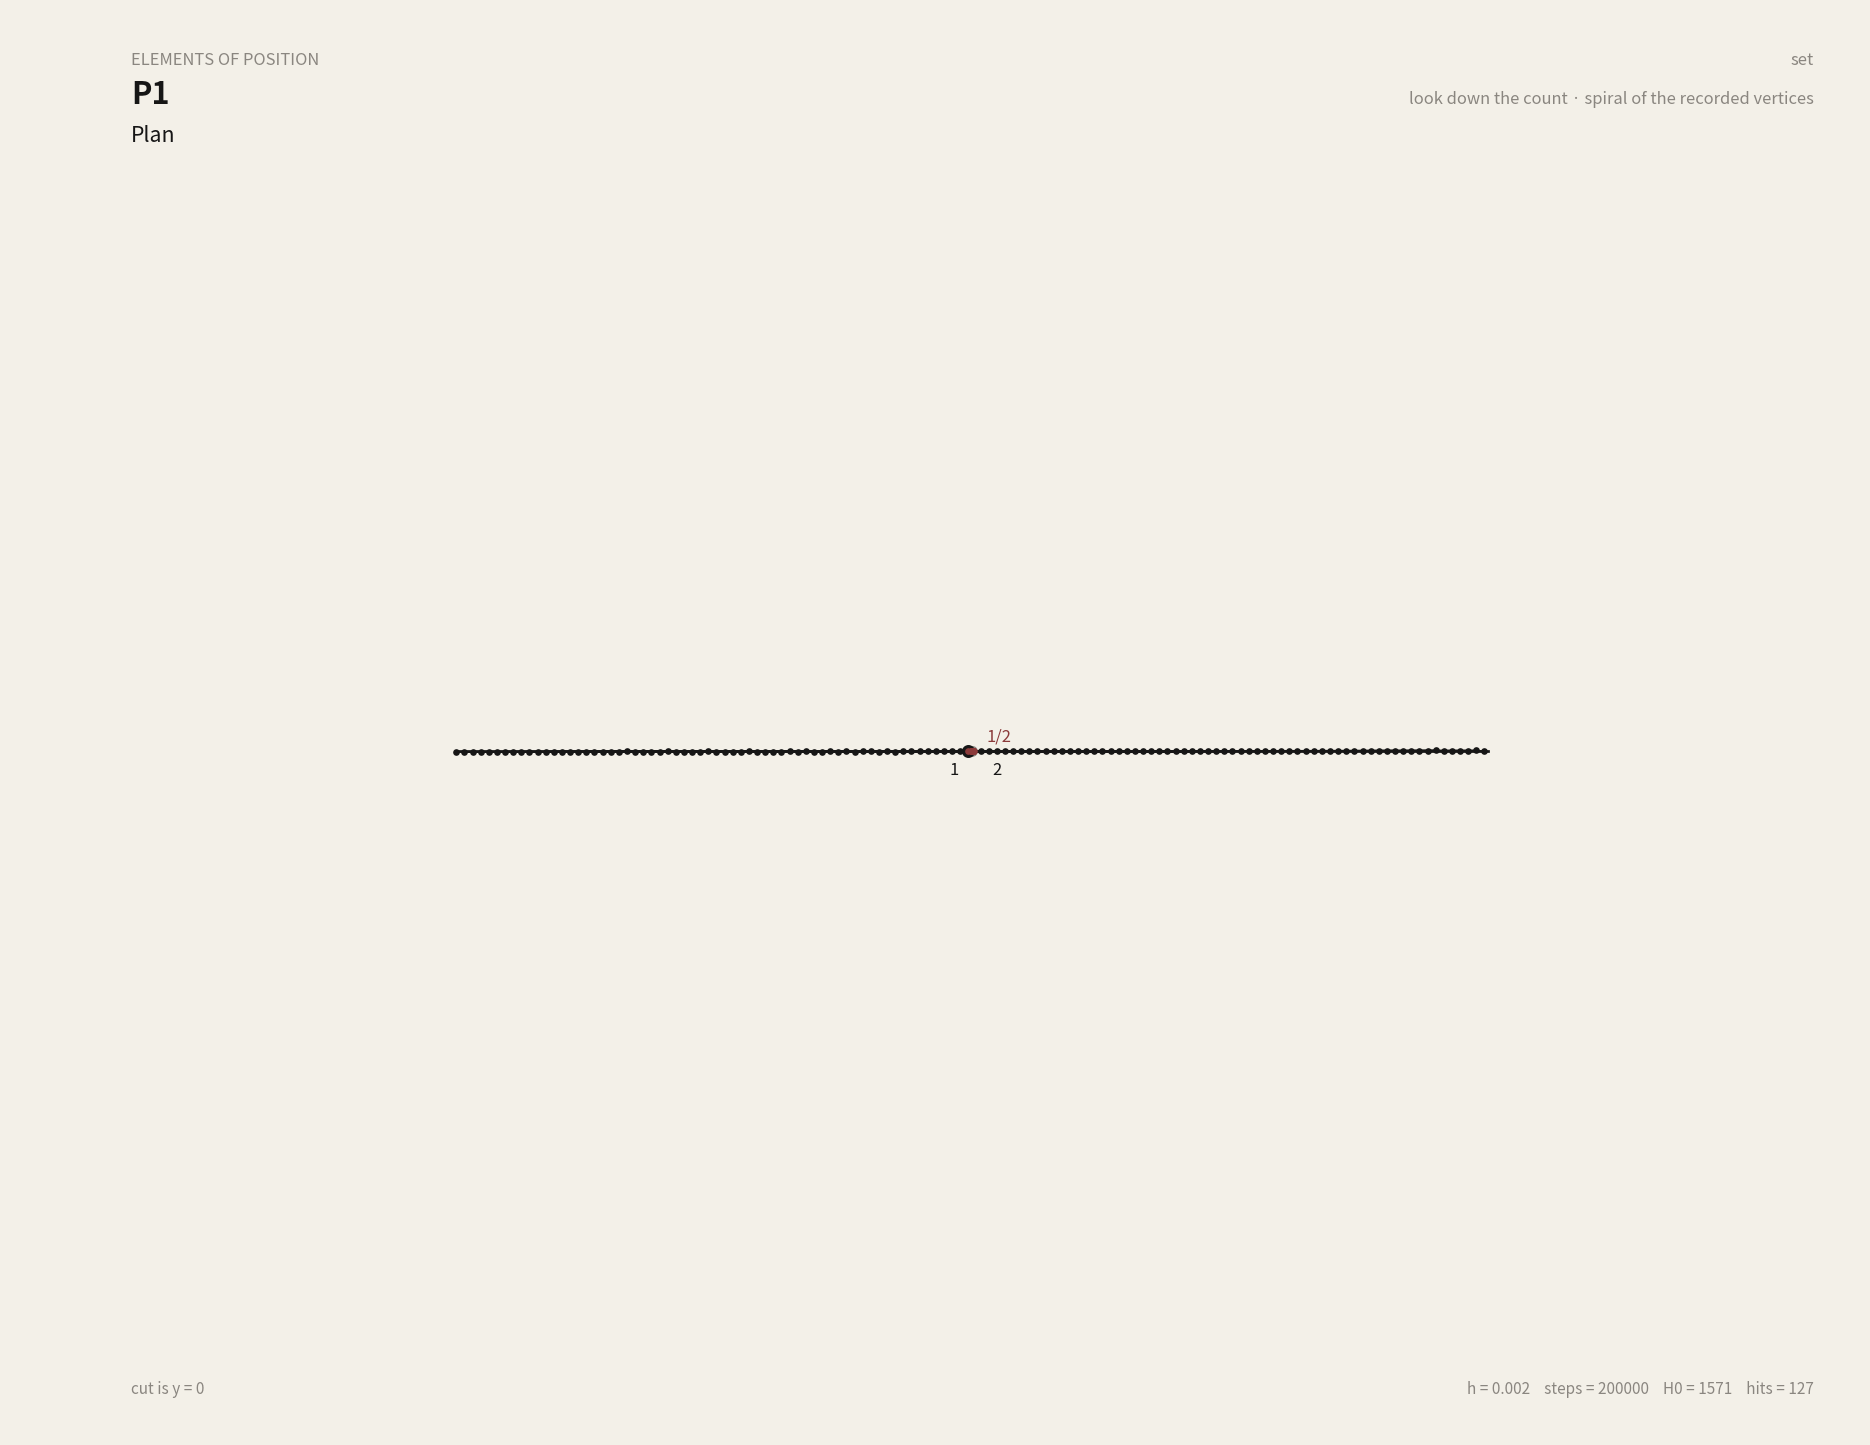
\includegraphics[width=0.92\textwidth]{P1_plan.png}
\caption{Sheet P1. Plan of the recorded hits. Outer locus in ink; inverse in the accent.
Hits sit on the cut, so the plan of \(P_m\) is nearly a line.
A spiral appears only when every step is drawn with radius growing as \(k/2\).
That is a later sampling of the same walk, not a second object.}
\end{figure}

\section{Four points}

\begin{proposition}
For every \(m>1\),
\(\bigl(1/m,\, m;\, 1,\, -1\bigr)=-1\).
\end{proposition}

The four points are the pair and the two marks the diameter already fixed.
This is the classical involution \(z\mapsto 1/z\) on the line.

The circle on diameter \(OP_m\) meets the unit circle at points whose foot on the ray of \(u_m\) is exactly \(Q_m\).
No idealization.
Checked on the recorded headings to machine precision.


\begin{figure}[htbp]
\centering
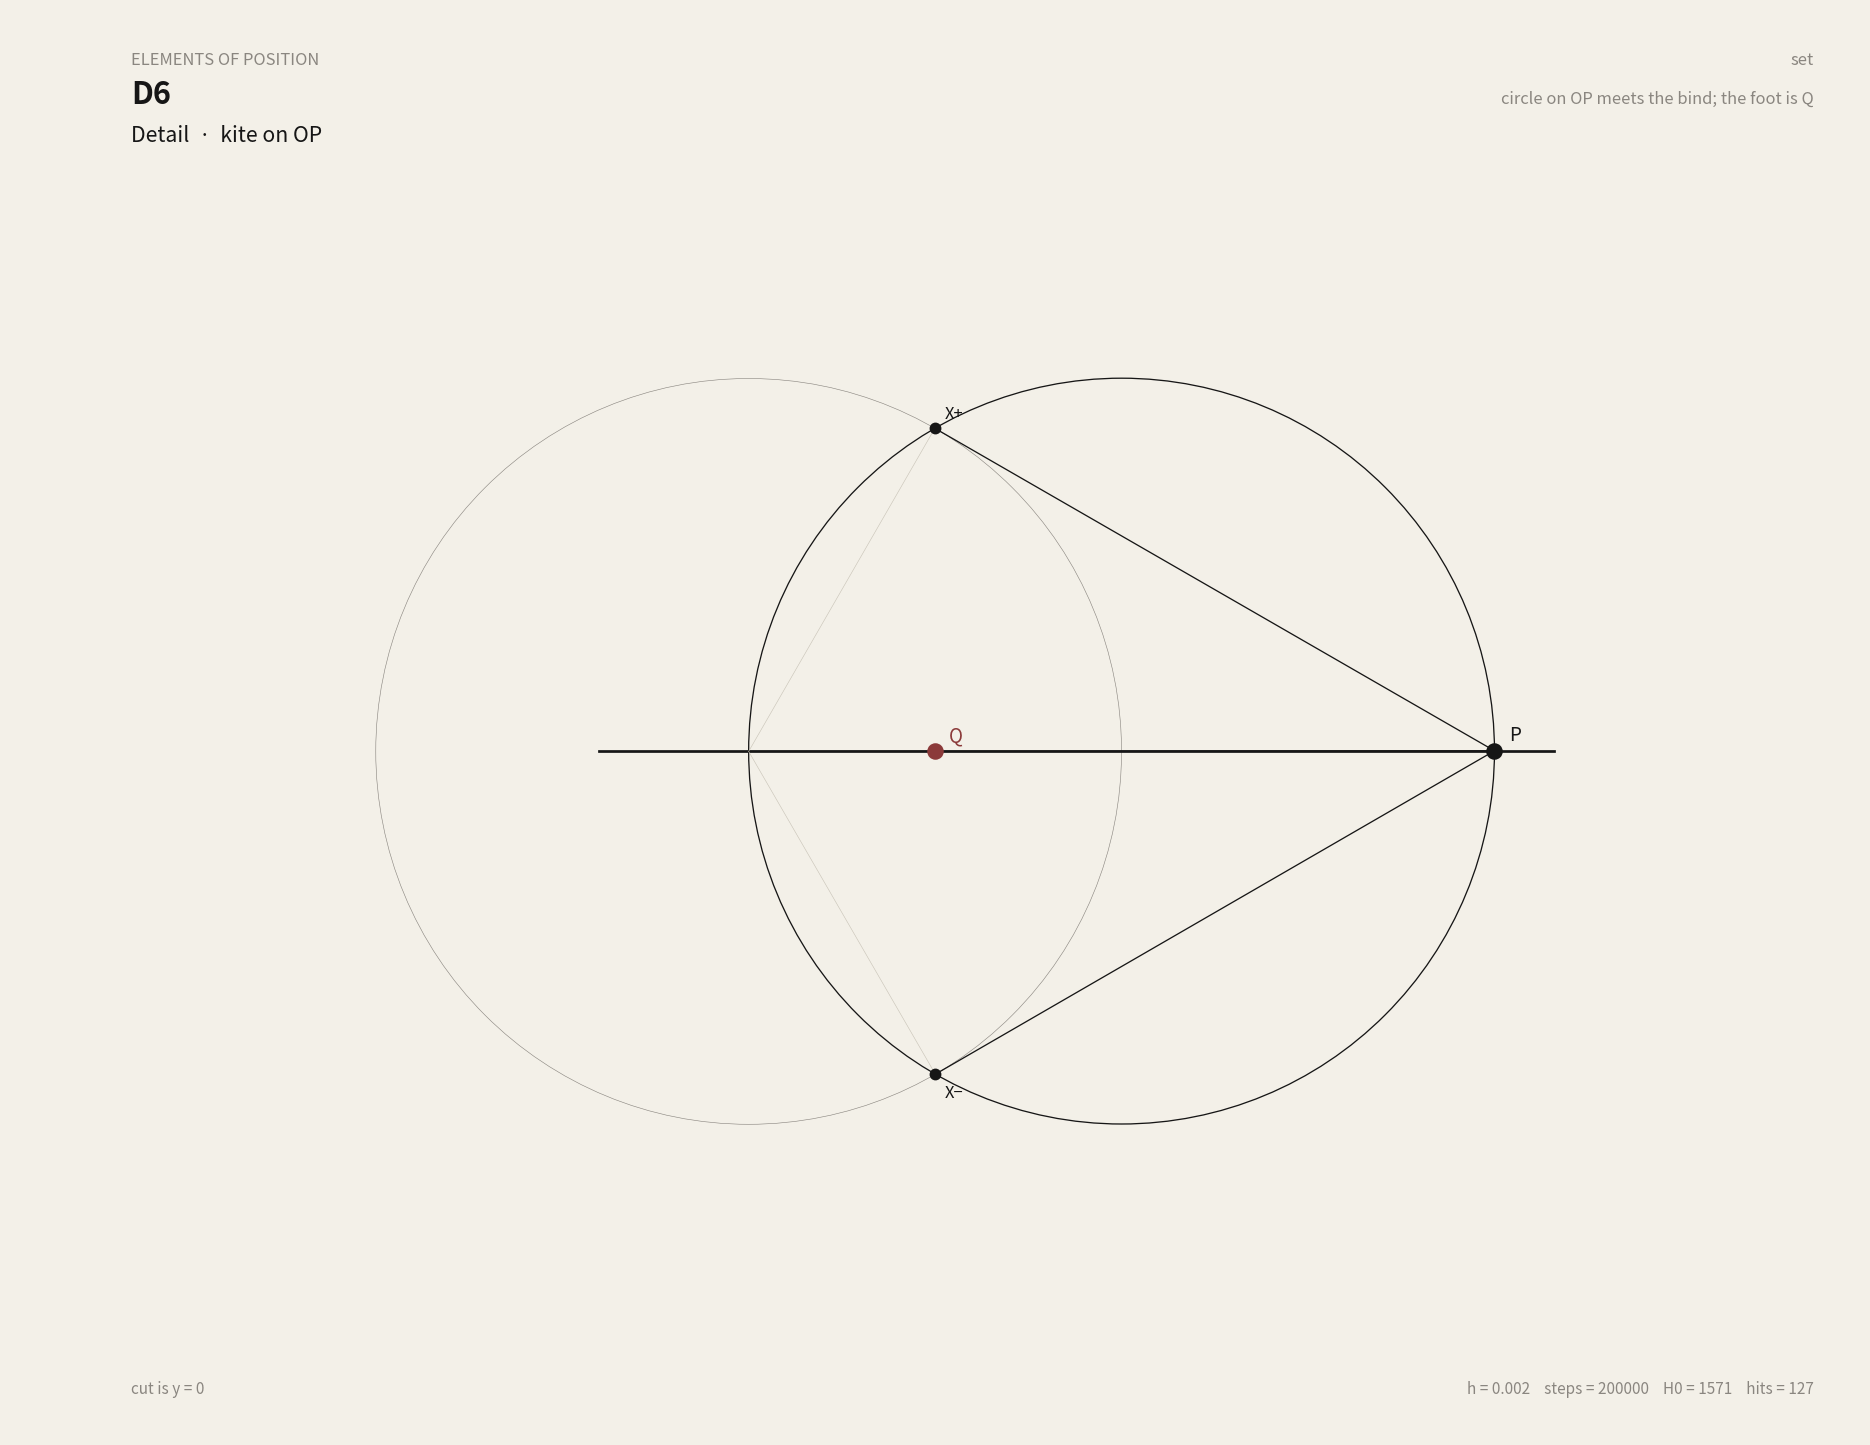
\includegraphics[width=0.92\textwidth]{D6_kite.png}
\caption{Sheet D6. Circle on $OP$ meeting the bind. The foot is $Q$.}
\end{figure}

\section{The count pays with two integers}

After the first hit the recorded run writes only two gap values: \(1570\) and \(1571\).
On \(127\) hits, \(1571\) occurs \(102\) times and \(1570\) occurs \(25\) times.
Mean gap times kick: \(3.14160630\).

A named comparison after the table exists:
\[
\lambda:=\frac{\pi}{\arctan h}=1570.798421,\qquad \{\lambda\}=0.798421.
\]

The walk cannot land on one length, so it writes both neighbors.
This is the discrete case of the three-distance theorem.


\begin{figure}[htbp]
\centering
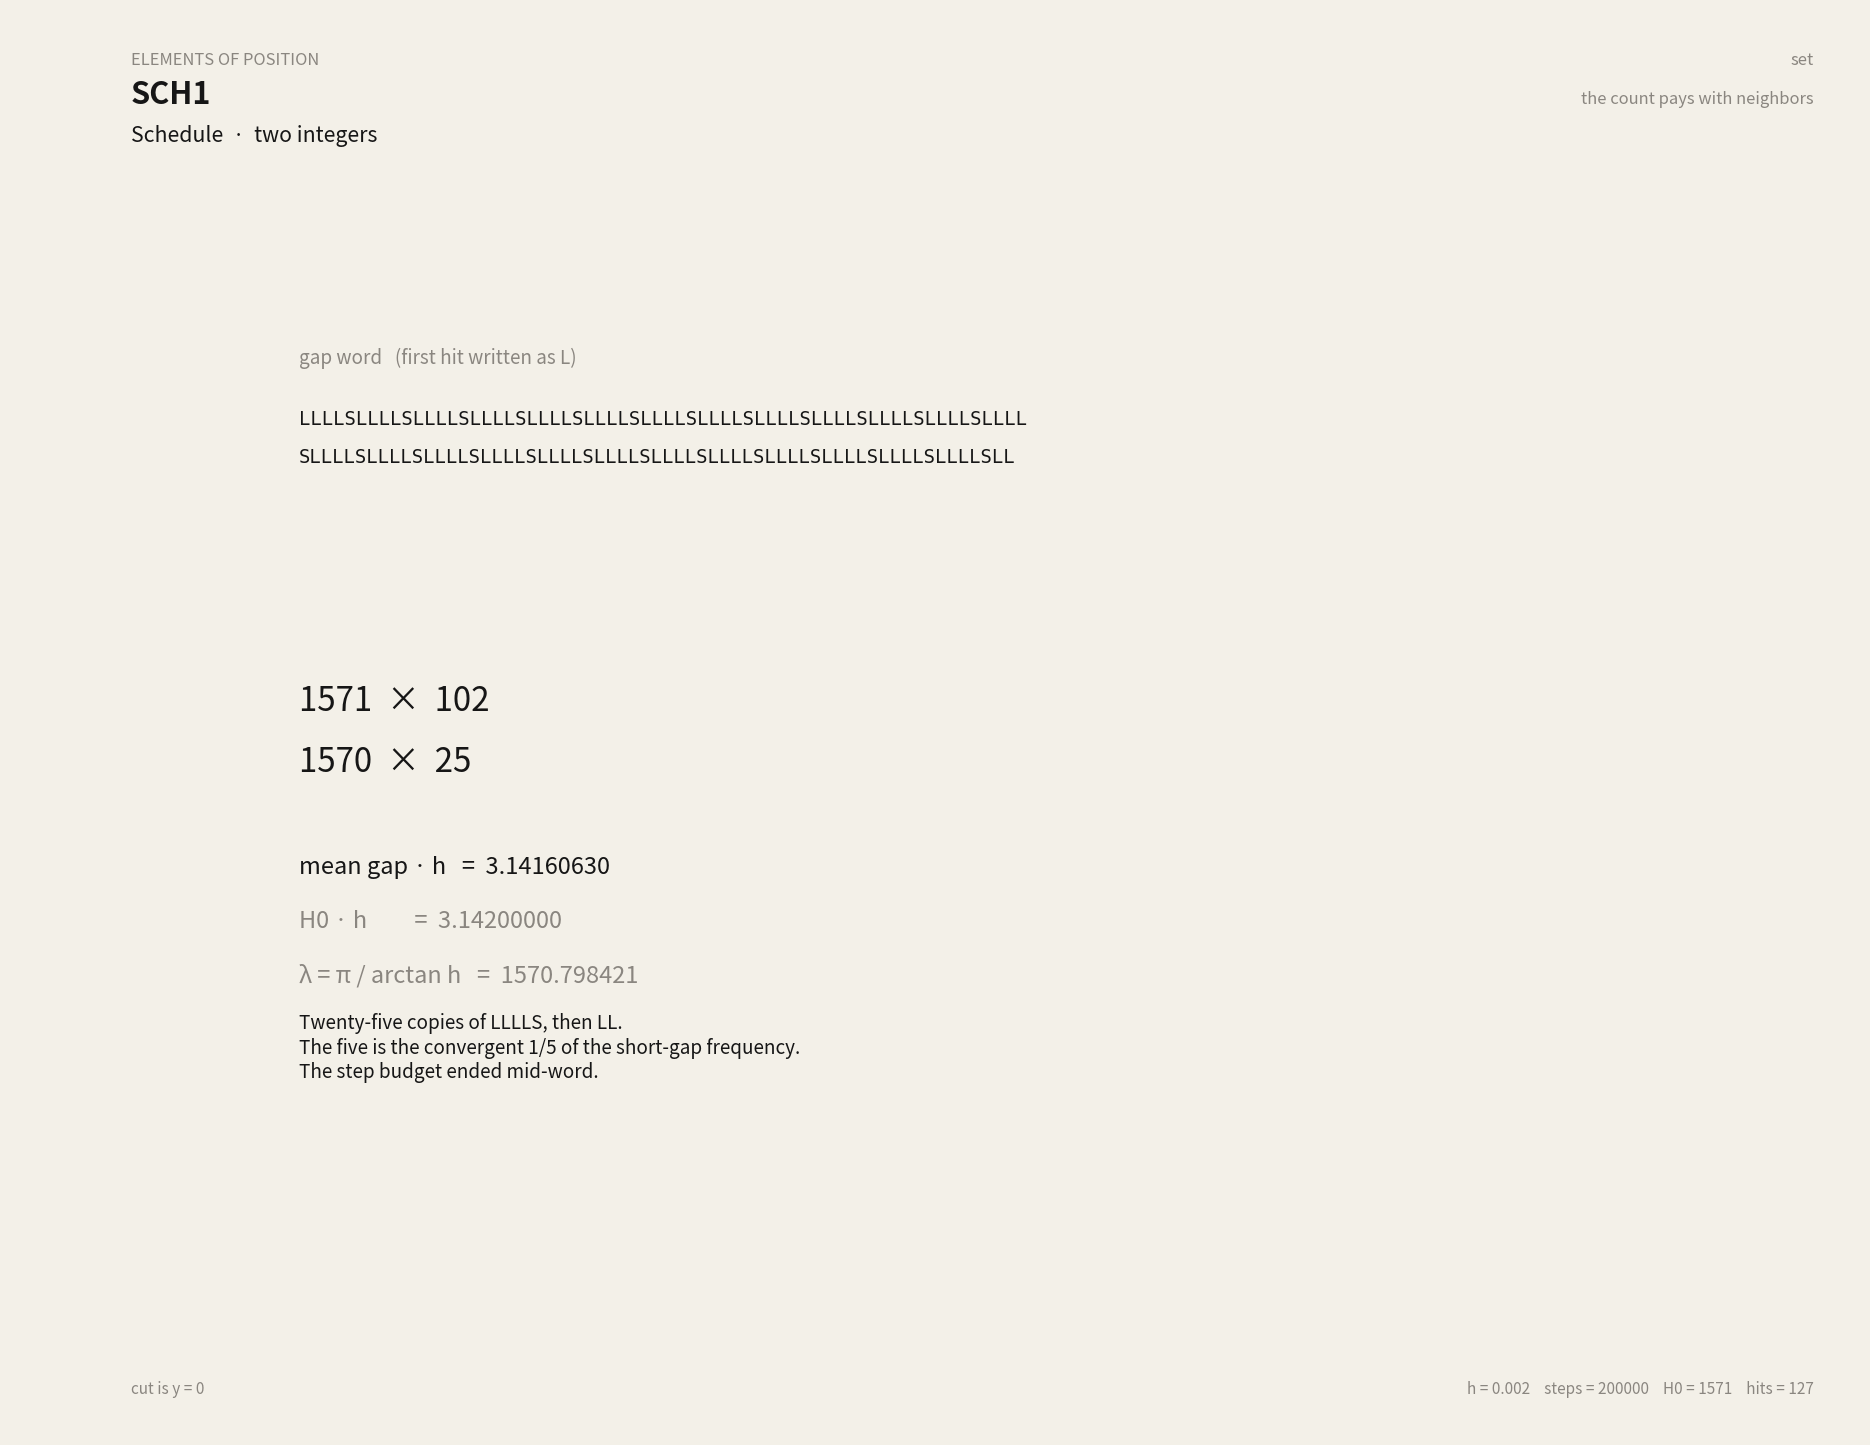
\includegraphics[width=0.92\textwidth]{SCH1_integers.png}
\caption{Sheet SCH1. Two gap integers on the recorded run.}
\end{figure}

\section{Two mixes}

\begin{observation}[Half-turn mix]
Choose \(h=\tan(\pi/n)\) for an integer \(n\ge 3\).
Then \(\lambda=n\) exactly, and every gap after the first hit equals \(n\).
Checked here: \(n=3,4,5,6,8\), one letter after the first hit.
At \(n=4\), \(h=1\), the square lands.
\end{observation}

\begin{observation}[Vertex mix]
Choose \(h=\tan(2\pi/n)\).
One elementary step is the central angle of the regular \(n\)-gon.
For \(n\ge 5\) that step is legal.
For \(n=4\) the tangent is a pole.
For \(n=3\) the tangent of \(2\pi/3\) is negative; it is not this series' positive kick.
\end{observation}

A hit is a half-turn.
A vertex step is \(2\pi/n\).
Steps per hit are therefore about \(n/2\), not \(n\).
At the pentagon vertex mix the recorded gaps are \(\{2,3\}\), not \(\{5\}\).
The vertices are still the pentagon: five steps from \((1,0)\) close with error \(3.4\times 10^{-17}\), sides equal to \(2\sin(\pi/5)\) with error \(0\).
Marriage of the two kernels (Part~IV) uses the vertex mix.
Exact closure of the gap word uses the half-turn mix.
They must not share a sentence that says ``at \(n=5\) the walk lands.''

\section{What stands}

Forced, once the operators are granted:
the step with no angle in either move;
a hit as a sign change;
the pair and the leftover, by Part~I;
\(P_m\) and \(Q_m\), and \(Q\) as inversion of \(P\);
the circle on \(OP\) with foot \(Q\), at every residual.

Reported from the named table:
two gap integers;
mean gap times kick next to \(\pi\);
\(H_0=1571\).

Not granted:
an angle as an argument of the step;
a landing on the cut;
the two mixes crushed into one kick;
a spiral treated as a different object from the hit plan.

Where is \(1\)?
It is still the lock.
The operators met themselves.
They did not land.

\end{document}
